\documentclass{minimal}
\usepackage{tikz}
%\usetikzlibrary{calc,trees,positioning,arrows,chains,shapes.geometric,decorations.pathreplacing,decorations.pathmorphing,shapes,matrix,shapes.symbols}
\usetikzlibrary{positioning}
\usetikzlibrary{shapes}

\begin{document}
\begin{center}
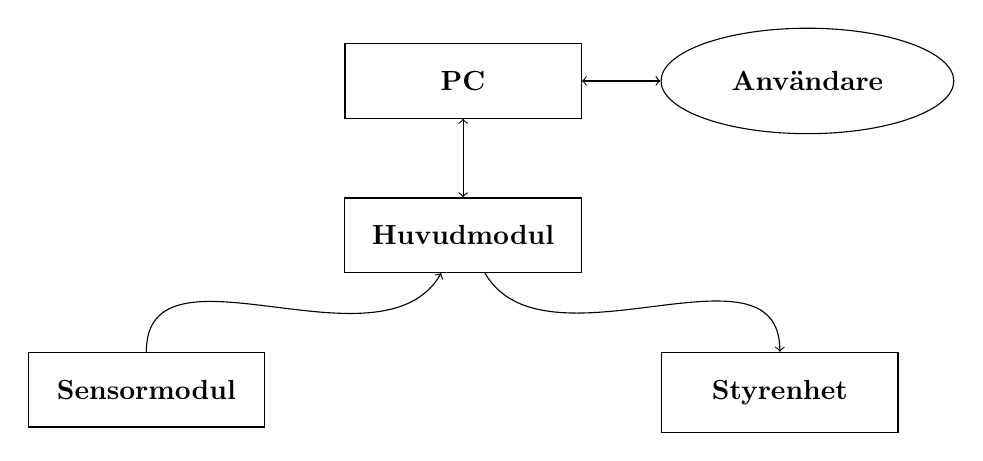
\begin{tikzpicture}[scale=1]
\tikzset{every node/.style={inner sep=10pt, minimum width=3 cm}}
%\draw[help lines,step=5mm,gray!20] (-5,-10) grid (5,0);
\node[draw, fill=white] (Huvudmodul)  {\textbf{Huvudmodul}};
\node[draw,below left= of Huvudmodul] (Sensormodul) {\textbf{Sensormodul}};
\node[draw,below right = of Huvudmodul] (Styrenhet) {\textbf{Styrenhet}};
\node[draw, above = of Huvudmodul] (PC) {\textbf{PC}};
\node[ellipse,draw, right = of PC] (Användare) {\textbf{Användare}};

\draw[->] (Huvudmodul) [out=300, in= 90] to (Styrenhet);
\draw[->] (Sensormodul) [out=90, in=240] to (Huvudmodul);
\draw[<->] (Huvudmodul) to (PC);
\draw[<->] (PC) to (Användare);
\end{tikzpicture}
\end{center}
\end{document}